\documentclass[12pt,a4,oneeside]{report}
\usepackage[top=.80in, bottom=.80in, left=1.1in, right=.80in, headsep=10pt ]{geometry}
\usepackage{setspace}
\usepackage[titletoc]{appendix}
\usepackage{amsmath}    
\usepackage{verbatim}   
\usepackage{color}      
 
\usepackage{hyperref}   
\usepackage{graphicx}
\usepackage{fancyhdr}
\usepackage{setspace}
\usepackage{multirow}
\usepackage{subfigure}
\usepackage[T1]{fontenc}
\usepackage{algorithm}
\usepackage{graphicx}
\usepackage{fancyhdr}
\usepackage{url}
\usepackage{array}
\usepackage{amssymb}
\usepackage{float}
\usepackage[utf8]{inputenc}
\usepackage{titlesec}
\usepackage{enumitem}
\usepackage{tabu}
\usepackage{hhline}
\usepackage{algpseudocode}
\usepackage{ragged2e}
% Additional packages for project content
\usepackage{booktabs}
\usepackage{longtable}
\usepackage{tabularx}
\usepackage{xcolor}
\usepackage{colortbl}
\usepackage{caption}
\usepackage{subcaption}
\usepackage{listings}
\usepackage{tcolorbox}
\usepackage{tikz}
\usepackage{pgfplots}
\pgfplotsset{compat=1.18}
\usetikzlibrary{shapes.geometric, arrows.meta, positioning, fit, backgrounds, decorations.pathreplacing}
\usepackage{microtype}
\usepackage{lmodern}
\usepackage{parskip}
\usepackage{mdframed}
\usepackage{cleveref}
% ─── Colours ────────────────────────────────────────────────────────────────
\definecolor{magnaRed}{RGB}{200,16,46}
\definecolor{magnaDark}{RGB}{35,31,32}
\definecolor{magnaGray}{RGB}{100,100,100}
\definecolor{magnaLightGray}{RGB}{245,245,245}
\definecolor{magnaBlue}{RGB}{0,84,166}
\definecolor{successGreen}{RGB}{0,128,0}
\definecolor{warningOrange}{RGB}{204,102,0}
\definecolor{tableHeader}{RGB}{200,16,46}
\definecolor{tableRowAlt}{RGB}{248,240,242}
\definecolor{codeBg}{RGB}{250,250,250}
% ─── Table helpers ───────────────────────────────────────────────────────────
\newcommand{\tableheadcolor}{\rowcolor{tableHeader}}
\newcommand{\tableheadfont}{\color{white}\bfseries}
% ─── Custom boxes ────────────────────────────────────────────────────────────
\tcbuselibrary{skins, breakable, listings}
\newtcolorbox{resultbox}[1][]{colback=magnaLightGray, colframe=magnaRed, title=#1, fonttitle=\bfseries\color{white},colbacktitle=magnaRed, boxrule=1pt, arc=4pt}
\newtcolorbox{findingbox}{colback=blue!5, colframe=magnaBlue,boxrule=0.8pt, arc=4pt, left=6pt, right=6pt}
\newtcolorbox{conclusionbox}{colback=green!5, colframe=successGreen,boxrule=0.8pt, arc=4pt, left=6pt, right=6pt}
\newtcolorbox{limitationbox}{colback=orange!5, colframe=warningOrange,boxrule=0.8pt, arc=4pt, left=6pt, right=6pt}
% ─── Listings ────────────────────────────────────────────────────────────────
\lstset{backgroundcolor=\color{codeBg},basicstyle=\ttfamily\small,breaklines=true,frame=single,rulecolor=\color{magnaGray},captionpos=b}




\setlength{\headheight}{14.5pt}
\addtolength{\topmargin}{-2.5pt}

\titleformat{\chapter}[display]
{\normalfont\huge\bfseries}{\chaptertitlename\ \thechapter}{18pt}{\Huge\centering}
\titlespacing*{\chapter}{0pt}{-15pt}{20pt}

\begin{document}
\onehalfspacing \input{certificate.tex}
\onehalfspacing \newpage
\pagestyle{empty}
\begin{figure}[h]
\centering

\includegraphics[scale=0.5]{images/logo.jpg}
\end{figure}

\begin{center}
{\large Department of Computer Science and Engineering}\\[4pt]
{\large 2025--2026}\\[12pt]
{\Large\bf CERTIFICATE}
\end{center}

\vspace{0.6cm}
\begin{justify}
This is to certify that the project entitled \textbf{``Inline Quality Control for Casting Cracks''} is a bonafide work carried out by the student team Sushanth Tiwari (01FE23BCS086), Sinchana S M (01FE23BCS192) and Akshata Shet (01FE23BEV035), in partial fulfillment of the completion of 6th semester Minor Project during the year 2025--2026. The project report has been approved as it satisfies the academic requirement with respect to the project work prescribed for the above said course.
\end{justify}

\vspace{1.2cm}
\begin{flushleft}
Neha Tarannum \hspace{8.5cm} Head, CSE\\[4pt]
(Guide, Assistant Professor) \hspace{6.8cm} Dr.\ Vijayalakshmi M.
\end{flushleft}

\vspace{1.2cm}
\begin{center}
{\large External Viva-Voce}
\end{center}

\vspace{0.8cm}
\begin{flushleft}
Name of the examiners \hspace{2.5cm} Signature with date\\[8pt]
1.\;------------------------------------------\hspace{1.5cm}----------------------\\[14pt]
2.\;------------------------------------------\hspace{1.5cm}----------------------
\end{flushleft}
\newpage

\onehalfspacing \chapter*{ABSTRACT}%
\begin{justify}
\addcontentsline{toc}{chapter}{ABSTRACT}

This project presents an automated surface defect detection system for High-Pressure Die Cast (HPDC) aluminium components, developed in partnership with Magna International. The primary objective is to detect and localise \textbf{Cracks} and \textbf{Cold Shuts} on casting surfaces using a deep learning-based object detection model, replacing labour-intensive and inconsistent manual visual inspection at production scale.

The dataset comprises 256 high-resolution HPDC casting images (4096$\times$3000 pixels) annotated in COCO polygon format. Exploratory data analysis revealed that crack bounding boxes occupy as little as 0.065\% of the total image area, making them extreme small objects that are unsuitable for full-image detection. A sliding-window patch-based training strategy was therefore adopted. The system uses \textbf{RF-DETR Medium} (Apache 2.0 licence), a Detection Transformer with a DINOv2 ViT-B backbone and multi-scale deformable attention decoder, selected over YOLO-family models due to commercial licensing constraints.

Over seven structured experiments, the pipeline was progressively refined through dataset balancing, crack-focused augmentation (horizontal flip), and patch size scaling from 768$\times$768 to 1024$\times$1024 pixels with 35\% overlap. The final best-performing configuration achieved an EMA mAP50-95 of \textbf{0.2379} and mAP50 of \textbf{0.4647}, representing an approximately 11\% relative improvement over the initial baseline. The key finding is that dataset engineering, particularly increasing patch size and overlap, had a greater impact on performance than any architectural change.

\end{justify}
\pagenumbering{roman}

\begin{flushleft}
\vspace{1cm}
\textsl{\textbf{Keywords:} HPDC Casting, Surface Defect Detection, RF-DETR, Object Detection, Deep Learning, DINOv2, Patch-Based Training, Crack Detection, Deformable DETR, Magna International.}
\end{flushleft}

\pagenumbering{roman}
 %write the abstract after completion of project
\onehalfspacing \chapter*{ACKNOWLEDGEMENT}

%\addcontentsline{toc}{chapter}{ACKNOWLEDGEMENT}

\begin{justify}

We would like to thank our faculty and management for their professional guidance towards
the completion of the minor project work. We take this opportunity to thank Dr. Ashok
Shettar, Pro-Chancellor, Dr. P.G Tewari, Vice-Chancellor and Dr. B.S.Anami, Registrar for
their vision and support. \\ \\
We also take this opportunity to thank Dr. Meena S.M, Professor and Dean of Faculty, SoCSE,
Dr. Vijayalakshmi M, Professor, Head of CSE for having provided us direction and facilitated
for enhancement of skills and academic growth. \\ \\
We thank our guide \textbf{Neha Tarannum}, Designation, Department of Computer Science \&
Engineering for the constant guidance during interaction and reviews. \\ \\
We extend our acknowledgment to the reviewers for critical suggestions and inputs. We also
thank the project coordinator Dr. Uday Kulkarni, Mr. Sunil V. Gurlahosur and reviewers for
their suggestions during the course of completion. We express gratitude to our beloved
parents for constant encouragement and support.

\end{justify}

\begin{flushright}
\vspace{3cm}
Sushanth Tiwari -- 01FE23BCS086\\
\indent\indent\indent\indent\indent\indent\indent\indent\indent\indent\indent\indent\indent\indent\indent\indent\indent\indent\indent
Sinchana S M -- 01FE23BCS192\\
\indent\indent\indent\indent\indent\indent\indent\indent\indent\indent\indent\indent\indent\indent\indent\indent\indent\indent\indent
Akshata Shet -- 01FE23BEV035\\
\end{flushright}
     %uncomment this for final report
\pagenumbering{roman}
\onehalfspacing \newpage
\normalsize
\pagestyle{plain}

\renewcommand{\contentsname}  {CONTENTS}
\renewcommand{\listfigurename}{LIST OF FIGURES}
\renewcommand{\listtablename} {LIST OF TABLES}

\tableofcontents
    \addcontentsline{toc}{chapter}{CONTENTS}

\listoftables
    \addcontentsline{toc}{chapter}{LIST OF TABLES}

\listoffigures
    \addcontentsline{toc}{chapter}{LIST OF FIGURES}

    
\cleardoublepage
\pagenumbering{arabic}

\onehalfspacing \pagestyle{fancy}

\fancyhf{}
\fancyhead[R]{\textit{\tiny{<<Project Title>>}}}

\lfoot{\textit{\tiny{School of Computer Science \& Engineering, KLE Technological University, Hubballi - 31.}}}
\rfoot{\tiny{\thepage}}

\renewcommand{\headrulewidth}{1pt}
\renewcommand{\footrulewidth}{1pt}

\fancypagestyle{plain}{%
\lfoot{ \textit{\tiny {School of Computer Science \& Engineering, KLE Technological University, Hubballi - 31}}}}
\onehalfspacing \chapter{INTRODUCTION}

\justify

\section{Preamble}

High-Pressure Die Casting (HPDC) is one of the dominant manufacturing processes for producing complex, near-net-shape aluminium components at high production rates. Molten aluminium is injected into hardened steel dies at pressures up to 1500 bar, producing parts with tight dimensional tolerances and good surface finish in cycle times of under a minute. The automotive sector relies heavily on HPDC for structural and powertrain components including engine housings, transmission cases, and structural brackets. Magna International, one of the world's largest automotive suppliers, operates large-scale HPDC production lines where hundreds of castings are produced every shift.

Despite its efficiency, the HPDC process is susceptible to several classes of surface and sub-surface defects. The most safety-critical are \textbf{Cracks} --- linear fractures that form during solidification or ejection and can propagate under service loads, leading to part failure. \textbf{Cold Shuts} (also called cold shots) arise when two metal flow fronts meet before fusing, creating a visible seam that weakens the part. \textbf{Heat checking} produces a fine network of surface cracks caused by thermal cycling of the die; unlike structural cracks, heat checking patterns are generally cosmetic and considered acceptable (OK) by Original Equipment Manufacturer (OEM) standards. \textbf{Porosity} introduces sub-surface voids that reduce fatigue life. Distinguishing NOK (not OK) structural cracks from OK heat-checking patterns is one of the core challenges in automated inspection.

Current end-of-line (EOL) quality control at Magna relies on two methods: manual visual inspection by trained operators, and periodic X-Ray analysis. This project, developed in direct partnership with Magna International, addresses the need for an automated, inline NDT alternative by building a deep learning-based surface defect detection system using the RF-DETR object detection model.

\section{Motivation}

The motivation for automating defect detection at Magna International is rooted in safety criticality, production scale, and the fundamental limitations of existing inspection methods.

\begin{itemize}[leftmargin=2em]
    \item \textbf{Safety criticality:} HPDC structural parts are used in load-bearing automotive applications. Undetected surface cracks can propagate under mechanical and thermal stress, ultimately causing part failure. OEM specifications mandate zero tolerance for cracks above a defined size threshold.

    \item \textbf{Production scale:} Inspecting every casting manually is impractical when several hundred parts are produced per shift. Human inspectors are subject to fatigue-induced inconsistency, and inspection accuracy degrades over time. Automated vision-based systems provide reproducible, fatigue-free inspection at machine speed.

    \item \textbf{Inadequacy of current methods:} Manual visual inspection is not 100\% reliable --- small or faint cracks on complex three-dimensional geometries are easily missed. X-Ray analysis, while highly reliable, is limited to approximately three parts per shift per machine due to cycle time constraints, is expensive to operate, and cannot provide 100\% coverage. Response time from X-Ray to production feedback is long, allowing defective batches to accumulate before corrective action is taken.

    \item \textbf{Need for automated NDT:} There is therefore a compelling industrial requirement for an alternative or parallel non-destructive testing (NDT) method capable of automated EOL inspection of all produced parts. A vision-based system operating on surface images can achieve full-coverage, low-latency defect flagging without the cost and cycle-time constraints of X-Ray.

    \item \textbf{Commercial deployment constraints:} Any model adopted by Magna must be deployable on production line hardware under a commercially permissive open-source licence. AGPL-3.0 licensed software (which includes the YOLO family) requires derivative commercial products to be released as open source, making it legally incompatible with Magna's deployment environment.
\end{itemize}

\section{Literature Study}

The problem of automated defect detection in industrial manufacturing has a rich prior literature spanning three broad phases: classical machine vision, convolutional neural networks, and transformer-based detection.

\textbf{Classical and hand-crafted feature methods:} Early systems for casting defect detection relied on manually engineered descriptors. Histogram of Oriented Gradients (HOG), Local Binary Patterns (LBP), and Gabor filter responses were computed from greyscale images and fed into Support Vector Machines (SVM) or AdaBoost classifiers \cite{xu2020}. Xu et al.\ \cite{xu2020} demonstrated relief-algorithm and AdaBoost-SVM combinations for internal casting crack detection. While effective in controlled conditions, these methods require careful feature engineering for each defect type and deteriorate rapidly as surface complexity or lighting variability increases.

\textbf{CNN-based detection and YOLO family:} Deep convolutional neural networks eliminated the need for hand-crafted features by learning hierarchical representations from labelled data. VGG \cite{simonyan2014} and ResNet \cite{he2016} became standard backbone architectures for industrial inspection tasks. The YOLO (You Only Look Once) family \cite{redmon2016, bochkovskiy2020, jocher2022} brought real-time single-stage detection, and YOLOv8 and YOLO11 were evaluated early in this project for their strong out-of-the-box performance. However, both are released under the AGPL-3.0 licence, which requires any commercial product incorporating YOLO components to release its derivative source code openly --- a condition incompatible with Magna International's proprietary production system. This licence constraint necessitated finding a commercially viable alternative.

\textbf{DETR lineage and RF-DETR:} Carion et al.\ \cite{carion2020} proposed DETR (Detection Transformer), which reformulated object detection as a direct set-prediction problem using a transformer encoder-decoder and bipartite Hungarian matching, eliminating anchor boxes and non-maximum suppression. Deformable DETR \cite{zhu2020} addressed DETR's slow convergence by introducing sparse deformable attention, greatly improving small-object performance and training efficiency. DINOv2 \cite{oquab2023} introduced self-supervised Vision Transformer (ViT) pretraining that produces rich, transferable visual features competitive with supervised counterparts. RF-DETR \cite{robinson2025}, released by Roboflow in 2025 under the Apache 2.0 licence, combines a DINOv2 ViT-B backbone with a multi-scale feature projector and deformable DETR decoder, achieving state-of-the-art real-time detection performance. Its Apache 2.0 licence makes it fully compatible with commercial industrial deployment, and its DINOv2 backbone is particularly well-suited to fine-tuning on small specialist datasets such as the one in this project.

\section{Problem Definition}

Magna International's HPDC production line requires a reliable, automated EOL inspection system for surface defect detection on cast aluminium components. In HPDC, multiple defect types occur on part surfaces: \textbf{Cracks} (linear fractures, NOK if above a critical size as defined by OEM specifications), \textbf{Cold Shuts} (incomplete fusion lines, generally NOK), \textbf{Heat Checking} (fine thermal crack networks, typically OK and distinguishable by pattern), and \textbf{Porosity} (voids, not always visible on surface images). The core challenge is detecting and classifying NOK cracks reliably while tolerating OK surface patterns.

Current EOL control at Magna consists of two methods, each with significant limitations. Human visual inspection, while experienced, is not 100\% reliable on complex curved geometries and is subject to fatigue and individual variability. X-Ray analysis is limited to approximately three parts per shift per machine due to its cycle time, is expensive to operate, and has a long feedback loop that prevents timely corrective action. Neither method provides 100\% automated coverage.

The problem addressed in this project is formally stated as follows: given a dataset of 256 high-resolution HPDC casting images (4096$\times$3000 pixels) with COCO polygon-level annotations for Crack and Cold Shut classes, train an object detection model that localises defects via bounding boxes, measured by COCO mAP50-95. A critical sub-challenge is that crack bounding boxes occupy less than 0.1\% of the total image area --- making them extreme small objects for which full-image detection is infeasible and a patch-based strategy is required \cite{lin2014}. Furthermore, all components must use commercially permissive licences (Apache 2.0/MIT/BSD) compatible with Magna's industrial deployment requirements, excluding the YOLO family.

\section{Objectives}

The following objectives govern the scope and success criteria of this project:

\begin{enumerate}[leftmargin=2em]
    \item \textbf{Analyse and characterise the HPDC casting defect dataset} to understand defect scale, distribution, class imbalance, and annotation quality. Establish that a patch-based pipeline is necessary from quantitative EDA findings.

    \item \textbf{Classify and localise surface defects} (Crack and Cold Shut) using a deep learning object detection model with bounding box output, achieving end-to-end detection without manual post-processing.

    \item \textbf{Build a patch-based data engineering pipeline} to handle extreme small-object detection, converting full 4096$\times$3000 images into 1024$\times$1024 overlapping patches with Shapely polygon-aware annotation clipping, enabling crack detection where crack area is less than 0.1\% of image area.

    \item \textbf{Evaluate and compare model performance} across structured experiments using COCO mAP50-95 as the primary metric, quantifying the individual contribution of patch size, overlap, dataset balancing, and augmentation to overall detection performance.

    \item \textbf{Validate a commercially deployable solution} using an open-source licence (Apache 2.0) compatible with industrial deployment at Magna International, demonstrating RF-DETR as a viable and legally compliant alternative to AGPL-3.0 licensed YOLO-family models.
\end{enumerate}

\onehalfspacing \chapter{Introduction}

\justify

Magna International is one of the world's largest automotive component suppliers, producing structural and powertrain parts via High-Pressure Die Casting (HPDC). In HPDC, molten aluminium is injected into reusable steel dies at extreme pressures, producing complex near-net-shape components at high production rates. The two primary defect classes targeted in this project are Cracks --- linear fractures posing structural safety risks --- and Cold Shuts --- flow lines where two metal fronts fail to fuse. Automated vision-based detection is critical for reliable, consistent quality assurance at production speed.

\section{Preamble (Provide Introduction of the project)}
\justify

This project develops an end-to-end automated surface defect detection system for HPDC aluminium castings in partnership with Magna International. The system uses RF-DETR Medium, a Detection Transformer with a DINOv2 ViT-B backbone, fine-tuned on a patch-based dataset derived from 256 high-resolution HPDC casting images. The core innovation is a sliding-window patch pipeline that converts full 4096$\times$3000 pixel images into 1024$\times$1024 training patches, making it possible to detect cracks that occupy less than 0.1\% of the image area --- a scale at which standard full-image detectors fail entirely.

The project is structured in two phases. Phase 1 (current) covers bounding box detection and localisation of Crack and Cold Shut defects. Phase 2 (deferred) will extend to pixel-level segmentation and physical crack length measurement in millimetres.

\section{Motivation}
\justify

The motivation for this project arises from a combination of industrial necessity and technical challenge:

\begin{itemize}[leftmargin=2em]
    \item \textbf{Safety criticality:} HPDC components are used in structural automotive applications. Undetected cracks can propagate under mechanical and thermal loads, leading to part failure and safety hazards downstream.
    \item \textbf{Production scale:} A single experienced inspector evaluating thousands of parts per shift introduces fatigue-induced inconsistency. Automated detection provides reproducible results at machine speed.
    \item \textbf{Extreme scale challenge:} Exploratory data analysis revealed that crack bounding boxes occupy as little as 0.065\% of the total image area (roughly $90\times90$ pixels on a 12.3~MP image). This makes crack detection one of the hardest small-object detection problems in industrial computer vision.
    \item \textbf{Commercial licensing:} YOLO-family models (versions 8 and beyond) use the AGPL-3.0 licence, which requires derivative commercial products to also be open-sourced --- incompatible with industrial deployment. RF-DETR (Apache 2.0) is the commercially viable alternative.
\end{itemize}

\section{Literature Study}
\justify

Automated defect detection in manufacturing has advanced substantially with deep convolutional neural networks. Traditional approaches relied on hand-crafted features --- HOG descriptors, LBP histograms, Gabor filters --- combined with classical classifiers such as SVM or AdaBoost \cite{xu2020}. Deep learning methods have supplanted these by learning hierarchical representations directly from labelled data.

The Detection Transformer (DETR) paradigm \cite{carion2020} reformulated object detection as a direct set prediction problem, eliminating hand-designed anchor boxes and non-maximum suppression. Deformable DETR \cite{zhu2020} improved convergence and small-object performance through sparse deformable attention. \textbf{RF-DETR} \cite{robinson2025} builds on this lineage with a DINOv2 ViT-B backbone \cite{oquab2023}, multi-scale feature projector, and deformable decoder, making it ideal for fine-tuning on small industrial datasets with challenging object scales. Xu et al.\ \cite{xu2020} demonstrated the viability of machine learning for internal casting crack detection, motivating this surface-defect extension.

\section{Problem Definition}
\justify

Given 256 high-resolution HPDC casting images (4096$\times$3000 pixels) annotated with COCO polygon-level bounding boxes for two defect classes (Crack and Cold Shut), the problem is defined as:

\begin{itemize}[leftmargin=2em]
    \item \textbf{Primary:} Train an object detection model that accurately detects and localises Crack and Cold Shut defects, measured by COCO mAP50-95 on a held-out test set.
    \item \textbf{Key constraint:} Crack bounding boxes occupy $<0.1\%$ of image area, making full-image detection infeasible. A patch-based sliding-window strategy is required.
    \item \textbf{Licence constraint:} The model must use a licence compatible with commercial deployment (Apache 2.0 preferred). YOLO-family models are excluded.
    \item \textbf{Phase 1 scope:} Bounding box detection only. Segmentation and crack length measurement are deferred to Phase 2.
\end{itemize}

\section{Objectives of the project}
\justify

\begin{enumerate}[leftmargin=2em]
    \item Detect and classify surface defects (Crack and Cold Shut) in HPDC casting images using a commercially deployable deep learning model.
    \item Produce accurate bounding box localisations suitable for downstream quality control actions.
    \item Establish a reproducible patch-based training pipeline for extreme small-object detection.
    \item Quantify the impact of dataset engineering choices (patch size, overlap, balancing, augmentation) on detection performance through structured experiments.
    \item Validate RF-DETR as an Apache 2.0 licensed alternative to YOLO, achieving EMA mAP50-95 $\geq$ 0.20 on the test set.
\end{enumerate}
 
\onehalfspacing \chapter{PROPOSED SYSTEM}

\justify

The proposed system is an end-to-end deep learning pipeline for automated surface defect detection in HPDC aluminium castings. It addresses the fundamental challenge of detecting extremely small defect regions (crack area $<$ 0.1\% of image) in high-resolution industrial images, using a commercially deployable detection transformer architecture.

\section{Description of Proposed System}
\justify

The proposed system operates as a two-stage pipeline:

\begin{enumerate}[leftmargin=2em]
    \item \textbf{Data Engineering Pipeline:} A sliding-window patch generator divides full 4096$\times$3000 HPDC images into 1024$\times$1024 overlapping patches (35\% overlap). Shapely-based polygon clipping ensures accurate annotation transfer to each patch. Dataset balancing and crack-focused augmentation (horizontal flip) are applied to improve training signal quality.

    \item \textbf{RF-DETR Detection Model:} Each patch is processed by RF-DETR Medium, a Detection Transformer with a DINOv2 ViT-B backbone. The model is fine-tuned on the patch dataset and produces bounding box predictions with class labels (Crack / Cold Shut) and confidence scores, without requiring non-maximum suppression.
\end{enumerate}

\begin{figure}[H]
\centering
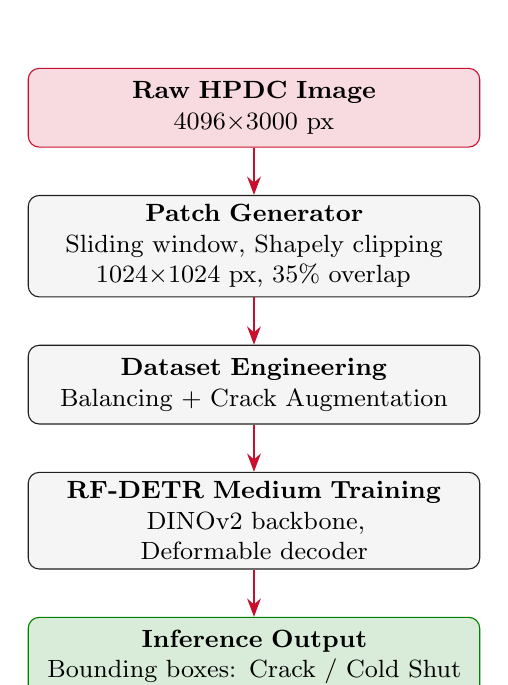
\begin{tikzpicture}[node distance=0.6cm and 2cm,
block/.style={rectangle, rounded corners=4pt, draw=magnaDark,
fill=magnaLightGray, text width=5.5cm,
minimum height=1cm, align=center, font=\small},
arrow/.style={-Stealth, thick, color=magnaRed}]
\node[block, fill=magnaRed!15, draw=magnaRed] (raw)
    {\textbf{Raw HPDC Image}\\4096$\times$3000 px};
\node[block, below=of raw] (patch)
    {\textbf{Patch Generator}\\Sliding window, Shapely clipping\\1024$\times$1024 px, 35\% overlap};
\node[block, below=of patch] (ds)
    {\textbf{Dataset Engineering}\\Balancing + Crack Augmentation};
\node[block, below=of ds] (train)
    {\textbf{RF-DETR Medium Training}\\DINOv2 backbone, Deformable decoder};
\node[block, fill=successGreen!15, draw=successGreen, below=of train] (infer)
    {\textbf{Inference Output}\\Bounding boxes: Crack / Cold Shut};
\draw[arrow] (raw)   -- (patch);
\draw[arrow] (patch) -- (ds);
\draw[arrow] (ds)    -- (train);
\draw[arrow] (train) -- (infer);
\end{tikzpicture}
\caption{High-level overview of the proposed HPDC defect detection system pipeline.}
\label{fig:system_overview}
\end{figure}

The Figure~\ref{fig:system_overview} shows the complete flow from raw casting image to defect detection output. The patch-based strategy is the core design decision that makes small-object crack detection feasible.

\section{Description of Target Users}
\justify

The system is designed for two primary user groups:

\begin{itemize}[leftmargin=2em]
    \item \textbf{Quality Control Engineers (Magna International):} End users who run inference on new casting images at the production line. They interact with the inference module via a simple command-line or GUI interface, receiving annotated images with bounding boxes highlighting detected defects.
    \item \textbf{ML Engineers / Research Team:} Users who operate the data engineering pipeline and training framework. They configure hyperparameters, run training experiments, and monitor mAP metrics to iterate on model performance.
\end{itemize}

A secondary stakeholder is Magna International's quality management team, who consume the defect detection results for process improvement and compliance reporting.

\section{Advantages / Applications of Proposed System}
\justify

\begin{itemize}[leftmargin=2em]
    \item \textbf{Automated and consistent inspection:} Removes inspector fatigue and subjective variability. Every casting is evaluated by the same model with reproducible confidence thresholds.
    \item \textbf{Extreme small-object detection:} The patch-based 1024$\times$1024 strategy with 35\% overlap is specifically engineered for cracks occupying $<$ 0.1\% of image area --- a capability not achievable with full-image detection.
    \item \textbf{Commercial deployment ready:} RF-DETR's Apache 2.0 licence permits unrestricted commercial use, deployment, and modification --- unlike YOLO-family models under AGPL-3.0.
    \item \textbf{End-to-end without NMS:} RF-DETR produces detections through bipartite matching, eliminating the need to tune non-maximum suppression thresholds.
    \item \textbf{Scalable to Phase 2:} The bounding box output of Phase 1 is a direct input to the planned Phase 2 segmentation and crack length measurement pipeline.
    \item \textbf{Reproducible experimentation:} Every experiment is fully documented with dataset statistics, training configurations, and evaluation metrics, enabling systematic improvement.
\end{itemize}

\section{Scope (Boundary of Proposed System)}
\justify

\textbf{In scope (Phase 1):}
\begin{itemize}[leftmargin=2em]
    \item Detection and classification of Crack and Cold Shut defects via bounding boxes.
    \item Patch-based sliding-window processing of HPDC images up to 4096$\times$3000 resolution.
    \item Training, evaluation, and checkpoint management for RF-DETR Medium.
    \item COCO-standard mAP evaluation on train/val/test splits.
\end{itemize}

\textbf{Out of scope (Phase 2, deferred):}
\begin{itemize}[leftmargin=2em]
    \item Pixel-level instance segmentation of crack regions.
    \item Morphological skeletonisation and centerline extraction.
    \item Crack length estimation in physical units (mm).
    \item Integration with Magna's production line control systems.
    \item Real-time video stream processing.
\end{itemize}

\onehalfspacing \chapter{SYSTEM DESIGN}

\justify

This chapter describes the architecture and design of the HPDC Defect Detection System, covering the full RF-DETR model architecture, data pipeline design, and dataset structure.

\section{Architecture of the System}
\justify

The system architecture consists of three major components: (1) the Data Engineering Pipeline, (2) the RF-DETR Detection Model, and (3) the Evaluation and Inference Engine. RF-DETR Medium uses a DINOv2 ViT-B backbone, a multi-scale projector neck, and a multi-scale deformable DETR decoder.

\begin{figure}[H]
\centering
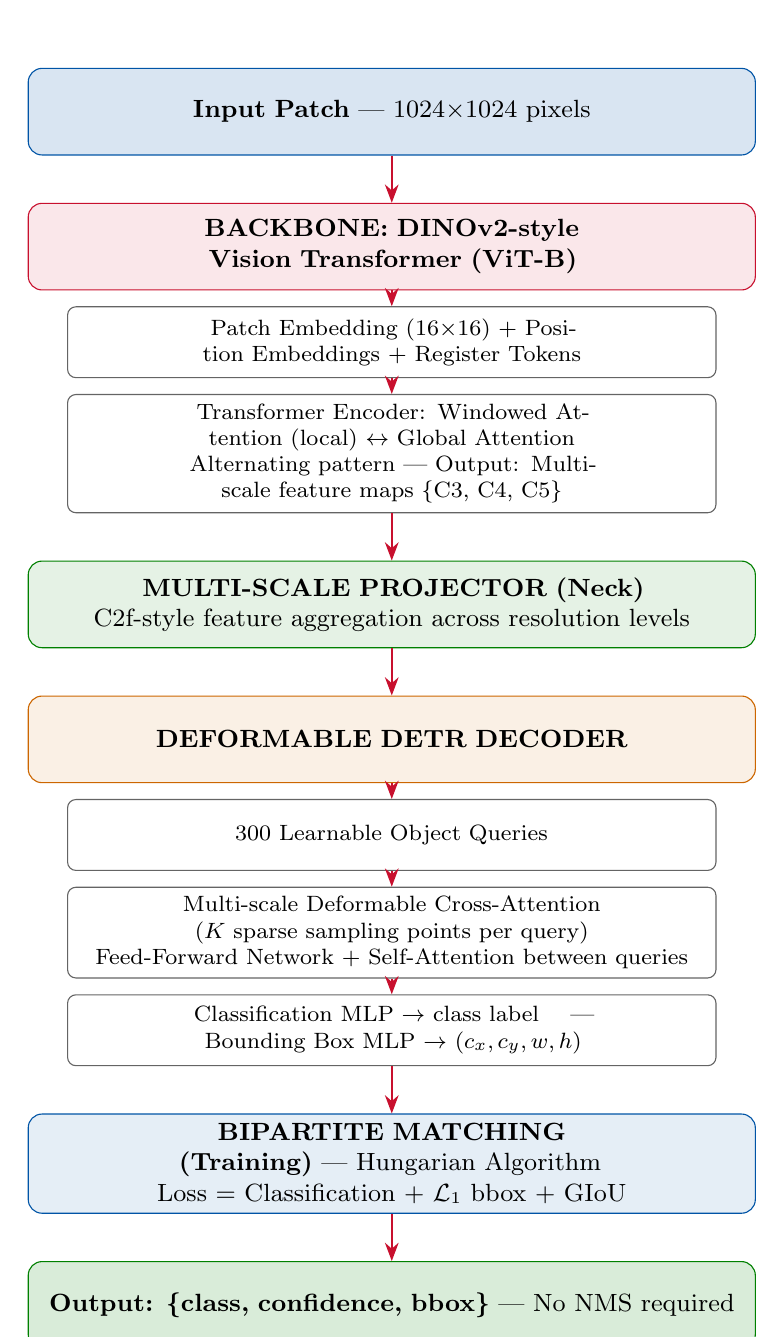
\begin{tikzpicture}[node distance=0.5cm,
mainblock/.style={rectangle, rounded corners=5pt, draw=magnaDark,
fill=magnaLightGray, text width=9cm,
minimum height=1.1cm, align=center, font=\small},
subblock/.style={rectangle, rounded corners=3pt, draw=magnaGray,
fill=white, text width=8cm,
minimum height=0.9cm, align=center, font=\footnotesize},
arrow/.style={-Stealth, thick, color=magnaRed}]

\node[mainblock, fill=magnaBlue!15, draw=magnaBlue] (input)
    {\textbf{Input Patch} --- 1024$\times$1024 pixels};
\node[mainblock, fill=magnaRed!10, draw=magnaRed, below=0.6cm of input] (backbone)
    {\textbf{BACKBONE: DINOv2-style Vision Transformer (ViT-B)}};
\node[subblock, below=0.2cm of backbone] (pembed)
    {Patch Embedding (16$\times$16) + Position Embeddings + Register Tokens};
\node[subblock, below=0.2cm of pembed] (vitblocks)
    {Transformer Encoder: Windowed Attention (local) $\leftrightarrow$ Global Attention\\
    Alternating pattern --- Output: Multi-scale feature maps \{C3, C4, C5\}};
\node[mainblock, fill=successGreen!10, draw=successGreen, below=0.6cm of vitblocks] (neck)
    {\textbf{MULTI-SCALE PROJECTOR (Neck)}\\C2f-style feature aggregation across resolution levels};
\node[mainblock, fill=warningOrange!10, draw=warningOrange, below=0.6cm of neck] (decoder)
    {\textbf{DEFORMABLE DETR DECODER}};
\node[subblock, below=0.2cm of decoder] (queries)
    {300 Learnable Object Queries};
\node[subblock, below=0.2cm of queries] (deformattn)
    {Multi-scale Deformable Cross-Attention ($K$ sparse sampling points per query)\\
    Feed-Forward Network + Self-Attention between queries};
\node[subblock, below=0.2cm of deformattn] (heads)
    {Classification MLP $\to$ class label \quad|\quad Bounding Box MLP $\to$ $(c_x, c_y, w, h)$};
\node[mainblock, fill=magnaBlue!10, draw=magnaBlue, below=0.6cm of heads] (matching)
    {\textbf{BIPARTITE MATCHING (Training)} --- Hungarian Algorithm\\
    Loss = Classification + $\mathcal{L}_1$ bbox + GIoU};
\node[mainblock, fill=successGreen!15, draw=successGreen, below=0.6cm of matching] (output)
    {\textbf{Output: \{class, confidence, bbox\}} --- No NMS required};

\draw[arrow] (input)      -- (backbone);
\draw[arrow] (backbone)   -- (pembed);
\draw[arrow] (pembed)     -- (vitblocks);
\draw[arrow] (vitblocks)  -- (neck);
\draw[arrow] (neck)       -- (decoder);
\draw[arrow] (decoder)    -- (queries);
\draw[arrow] (queries)    -- (deformattn);
\draw[arrow] (deformattn) -- (heads);
\draw[arrow] (heads)      -- (matching);
\draw[arrow] (matching)   -- (output);
\end{tikzpicture}
\caption{RF-DETR Medium complete architecture. Each patch is processed end-to-end from DINOv2 backbone through deformable decoder to produce detections without NMS.}
\label{fig:rfdetr_arch}
\end{figure}

\section{Class Diagram (with Brief Explanation)}
\justify

The system is organised into four primary Python classes. The \texttt{PatchGenerator} handles sliding-window extraction and Shapely polygon clipping. The \texttt{DatasetBuilder} applies balancing and augmentation. The \texttt{RFDETRTrainer} wraps the RF-DETR training loop with EMA tracking. The \texttt{DefectDetector} handles inference on full images.

\begin{figure}[H]
\centering
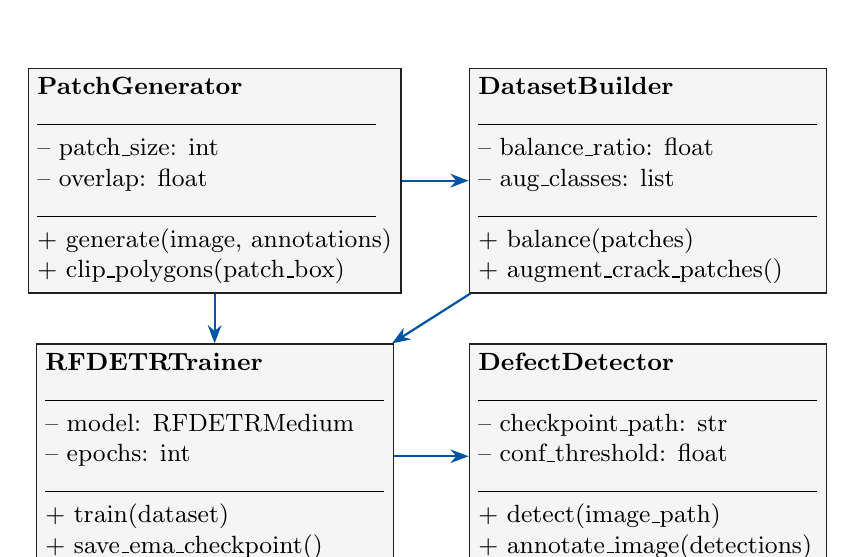
\begin{tikzpicture}[
    classbox/.style={rectangle, draw=magnaDark, fill=magnaLightGray,
    minimum width=4.5cm, font=\small},
    arrow/.style={-Stealth, thick, color=magnaBlue}
]
% PatchGenerator
\node[classbox, minimum height=2.2cm, align=left] (pg) at (0,0) {
    \textbf{PatchGenerator}\\
    \rule{4.3cm}{0.4pt}\\
    -- patch\_size: int\\
    -- overlap: float\\
    \rule{4.3cm}{0.4pt}\\
    + generate(image, annotations)\\
    + clip\_polygons(patch\_box)
};
% DatasetBuilder
\node[classbox, minimum height=2.2cm, align=left] (db) at (5.5,0) {
    \textbf{DatasetBuilder}\\
    \rule{4.3cm}{0.4pt}\\
    -- balance\_ratio: float\\
    -- aug\_classes: list\\
    \rule{4.3cm}{0.4pt}\\
    + balance(patches)\\
    + augment\_crack\_patches()
};
% RFDETRTrainer
\node[classbox, minimum height=2.2cm, align=left] (tr) at (0,-3.5) {
    \textbf{RFDETRTrainer}\\
    \rule{4.3cm}{0.4pt}\\
    -- model: RFDETRMedium\\
    -- epochs: int\\
    \rule{4.3cm}{0.4pt}\\
    + train(dataset)\\
    + save\_ema\_checkpoint()
};
% DefectDetector
\node[classbox, minimum height=2.2cm, align=left] (dd) at (5.5,-3.5) {
    \textbf{DefectDetector}\\
    \rule{4.3cm}{0.4pt}\\
    -- checkpoint\_path: str\\
    -- conf\_threshold: float\\
    \rule{4.3cm}{0.4pt}\\
    + detect(image\_path)\\
    + annotate\_image(detections)
};

\draw[arrow] (pg) -- (db);
\draw[arrow] (db) -- (tr);
\draw[arrow] (tr) -- (dd);
\draw[arrow] (pg) -- (tr);
\end{tikzpicture}
\caption{Simplified class diagram of the four main system components.}
\label{fig:class_diagram}
\end{figure}

\section{Sequence Diagram (with Brief Explanation)}
\justify

The sequence diagram below illustrates the inference flow: a quality engineer submits an image, the system generates patches, runs RF-DETR on each patch, and returns annotated detections.

\begin{figure}[H]
\centering
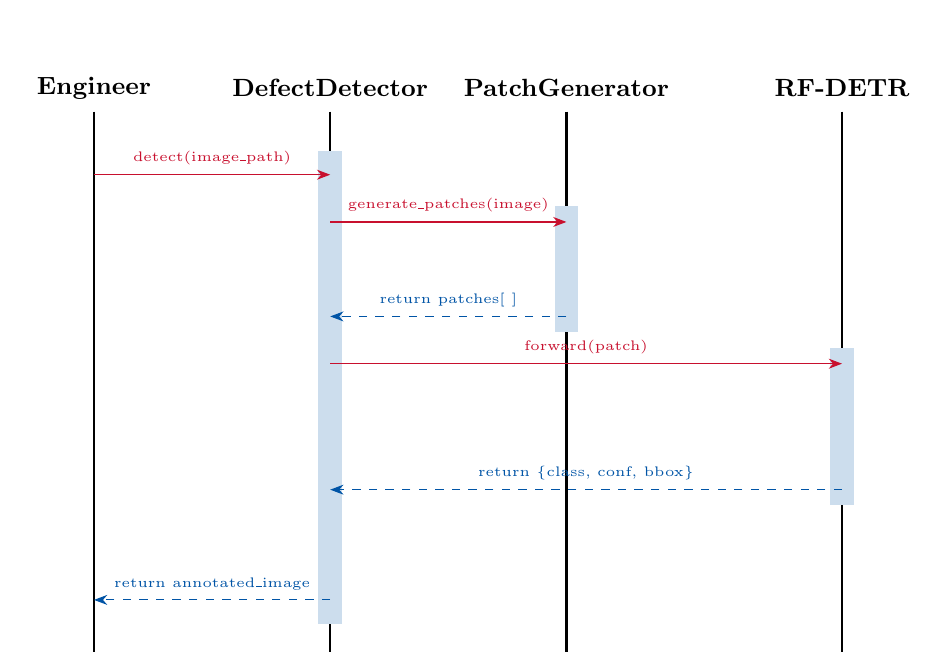
\begin{tikzpicture}[font=\small]
% Lifelines
\draw[thick] (0,0) -- (0,-7); \node at (0,0.3) {\textbf{Engineer}};
\draw[thick] (3,0) -- (3,-7); \node at (3,0.3) {\textbf{DefectDetector}};
\draw[thick] (6,0) -- (6,-7); \node at (6,0.3) {\textbf{PatchGenerator}};
\draw[thick] (9.5,0) -- (9.5,-7); \node at (9.5,0.3) {\textbf{RF-DETR}};

% Activations
\fill[magnaBlue!20] (2.85,-0.5) rectangle (3.15,-6.5);
\fill[magnaBlue!20] (5.85,-1.2) rectangle (6.15,-2.8);
\fill[magnaBlue!20] (9.35,-3.0) rectangle (9.65,-5.0);

% Messages
\draw[-Stealth, magnaRed] (0,-0.8) -- (3,-0.8) node[midway, above, font=\tiny] {detect(image\_path)};
\draw[-Stealth, magnaRed] (3,-1.4) -- (6,-1.4) node[midway, above, font=\tiny] {generate\_patches(image)};
\draw[-Stealth, dashed, magnaBlue] (6,-2.6) -- (3,-2.6) node[midway, above, font=\tiny] {return patches[ ]};
\draw[-Stealth, magnaRed] (3,-3.2) -- (9.5,-3.2) node[midway, above, font=\tiny] {forward(patch)};
\draw[-Stealth, dashed, magnaBlue] (9.5,-4.8) -- (3,-4.8) node[midway, above, font=\tiny] {return \{class, conf, bbox\}};
\draw[-Stealth, dashed, magnaBlue] (3,-6.2) -- (0,-6.2) node[midway, above, font=\tiny] {return annotated\_image};
\end{tikzpicture}
\caption{Sequence diagram for the defect detection inference flow.}
\label{fig:sequence_diagram}
\end{figure}

\section{ER Diagram and Schema (if applicable)}
\justify

The system does not use a relational database. Data is stored as COCO-format JSON files and PNG image patches on the filesystem. The logical schema is as follows:

\begin{table}[H]
\centering
\caption{COCO JSON Logical Schema}
\begin{tabular}{lll}
\toprule
\rowcolor{tableHeader}\tableheadfont Entity & \tableheadfont Key Fields & \tableheadfont Relationship \\
\midrule
Image           & id, file\_name, width, height & 1:N with Annotations \\
\rowcolor{tableRowAlt}Annotation      & id, image\_id, category\_id, bbox, segmentation & N:1 with Image \\
Category        & id, name (Crack / Cold Shut) & 1:N with Annotations \\
\bottomrule
\end{tabular}
\end{table}

\section{State Transition Diagram (if applicable)}
\justify

The training process transitions through well-defined states as shown below:

\begin{figure}[H]
\centering
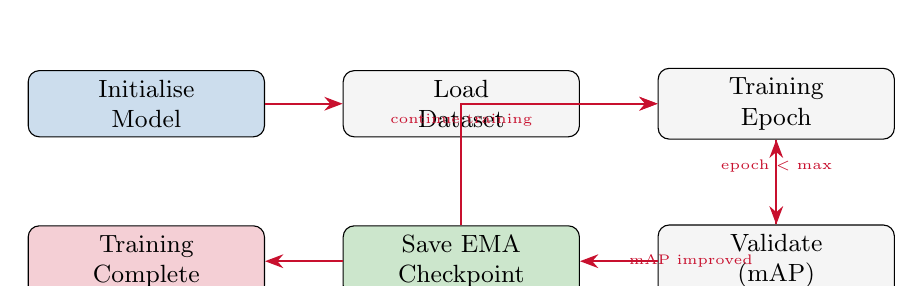
\begin{tikzpicture}[
    state/.style={draw, rounded corners, fill=magnaLightGray, minimum width=3cm, minimum height=0.8cm, font=\small, align=center},
    arrow/.style={-Stealth, thick, color=magnaRed}
]
\node[state, fill=magnaBlue!20] (init) at (0,0) {Initialise\\Model};
\node[state] (load) at (4,0) {Load\\Dataset};
\node[state] (train) at (8,0) {Training\\Epoch};
\node[state] (eval) at (8,-2) {Validate\\(mAP)};
\node[state, fill=successGreen!20] (save) at (4,-2) {Save EMA\\Checkpoint};
\node[state, fill=magnaRed!20] (done) at (0,-2) {Training\\Complete};

\draw[arrow] (init)  -- (load);
\draw[arrow] (load)  -- (train);
\draw[arrow] (train) -- (eval);
\draw[arrow] (eval)  -- node[right, font=\tiny] {mAP improved} (save);
\draw[arrow] (eval)  -- node[above, font=\tiny, text width=2cm, align=center] {epoch $<$ max} (train);
\draw[arrow] (save)  -- (done);
\draw[arrow] (save)  |- node[below, font=\tiny] {continue training} (train);
\end{tikzpicture}
\caption{State transition diagram for the RF-DETR training process.}
\end{figure}

\section{Dataset Description}
\justify

\begin{table}[H]
\centering
\caption{Original Dataset Summary}
\begin{tabular}{lc}
\toprule
\rowcolor{tableHeader}\tableheadfont Parameter & \tableheadfont Value \\
\midrule
Dataset name       & Cast\_Cracks\_Annotated\_Coco \\
\rowcolor{tableRowAlt}Training images    & 173 \\
Validation images  & 50 \\
\rowcolor{tableRowAlt}Test images        & 33 \\
\textbf{Total images} & \textbf{256} \\
\rowcolor{tableRowAlt}Image resolution   & 4096 $\times$ 3000 pixels \\
Annotation format  & COCO JSON (polygon-level) \\
\rowcolor{tableRowAlt}Defect classes     & Crack, Cold Shut \\
\bottomrule
\end{tabular}
\end{table}

\begin{table}[H]
\centering
\caption{Patch Dataset Summary (Final --- Experiment 7)}
\begin{tabular}{lcc}
\toprule
\rowcolor{tableHeader}\tableheadfont Split & \tableheadfont Images & \tableheadfont Annotations \\
\midrule
Train       & 2,939 & 2,743 \\
\rowcolor{tableRowAlt}Validation  & 750   & 705 \\
Test        & 495   & 596 \\
\rowcolor{tableRowAlt}\textbf{Total} & \textbf{4,184} & \textbf{4,044} \\
\bottomrule
\end{tabular}
\end{table}

Key EDA findings: the median crack bounding box occupies $\approx$0.065\% of the full image area (roughly $90\times90$ pixels on a 12.3~MP image), confirming that patch-based training is essential. Cold Shut objects are approximately $2\times$ larger than cracks on average, explaining the consistent per-class performance gap.

\onehalfspacing \chapter{IMPLEMENTATION}

\justify

This chapter describes the implementation methodology and key modules of the HPDC Defect Detection System. The implementation is divided into three functional stages: data engineering (patch generation, balancing, augmentation), model training (RF-DETR fine-tuning), and inference.

\section{Proposed Methodology}

The core methodology is a \textbf{patch-based sliding-window training pipeline} designed specifically for extreme small-object detection. Since crack bounding boxes occupy less than 0.1\% of the full image area, full-image training is infeasible. The approach divides each full HPDC image into overlapping 1024$\times$1024 patches, with Shapely polygon-aware annotation clipping to preserve accurate ground-truth boundaries.

\begin{figure}[H]
\centering
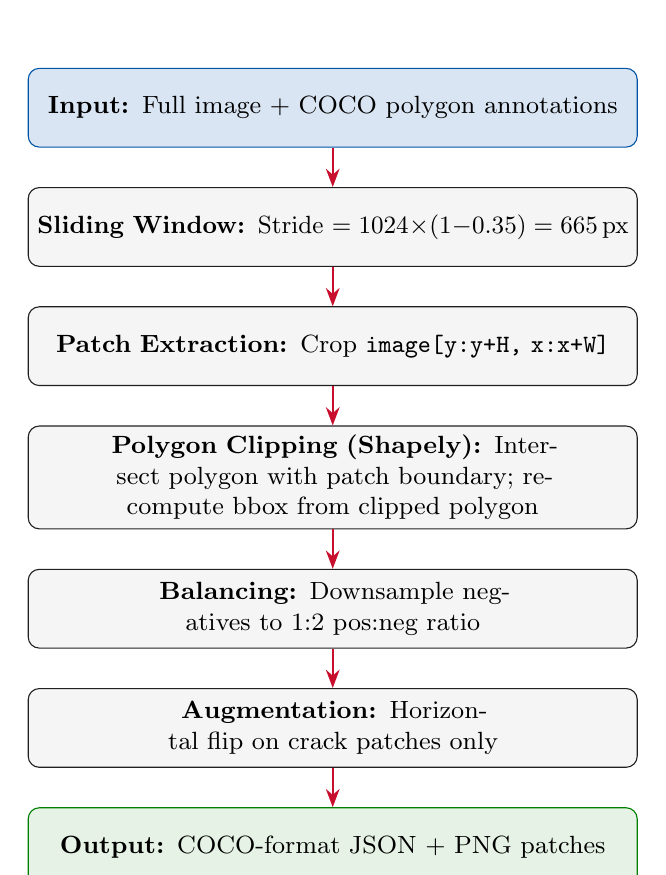
\begin{tikzpicture}[node distance=0.5cm,
block/.style={rectangle, rounded corners=4pt, draw=magnaDark,
fill=magnaLightGray, text width=7.5cm,
minimum height=1cm, align=center, font=\small},
arrow/.style={-Stealth, thick, color=magnaRed}]

\node[block, fill=magnaBlue!15, draw=magnaBlue] (input)
    {\textbf{Input:} Full image + COCO polygon annotations};
\node[block, below=0.5cm of input] (stride)
    {\textbf{Sliding Window:} Stride $= 1024 \times (1 - 0.35) = 665$\,px};
\node[block, below=0.5cm of stride] (extract)
    {\textbf{Patch Extraction:} Crop \texttt{image[y:y+H, x:x+W]}};
\node[block, below=0.5cm of extract] (shapely)
    {\textbf{Polygon Clipping (Shapely):} Intersect polygon with patch boundary;
    recompute bbox from clipped polygon};
\node[block, below=0.5cm of shapely] (balance)
    {\textbf{Balancing:} Downsample negatives to 1:2 pos:neg ratio};
\node[block, below=0.5cm of balance] (aug)
    {\textbf{Augmentation:} Horizontal flip on crack patches only};
\node[block, fill=successGreen!10, draw=successGreen, below=0.5cm of aug] (output)
    {\textbf{Output:} COCO-format JSON + PNG patches};

\draw[arrow] (input)   -- (stride);
\draw[arrow] (stride)  -- (extract);
\draw[arrow] (extract) -- (shapely);
\draw[arrow] (shapely) -- (balance);
\draw[arrow] (balance) -- (aug);
\draw[arrow] (aug)     -- (output);
\end{tikzpicture}
\caption{Proposed methodology flowchart: patch-based data engineering pipeline.}
\label{fig:methodology}
\end{figure}

The EMA (Exponential Moving Average) training strategy smooths weight updates across epochs:
\begin{equation}
\boldsymbol{\theta}_{\text{EMA}} = \alpha \cdot \boldsymbol{\theta}_{\text{EMA}} + (1-\alpha) \cdot \boldsymbol{\theta}_{\text{current}}
\end{equation}
where $\alpha$ is the decay factor (typically 0.9999). EMA weights consistently outperformed instantaneous weights across all experiments.

\section{Description of Modules}

\subsection*{Module 1: Patch Generator}

\begin{itemize}[leftmargin=2em, topsep=2pt]
    \item \textbf{Input:} Full HPDC image (4096$\times$3000 PNG), COCO annotation JSON
    \item \textbf{Output:} Set of 1024$\times$1024 PNG patches + updated COCO JSON with clipped annotations
    \item \textbf{Description:} Enumerates sliding-window positions with stride 665 px. For each patch, clips all polygon annotations using Shapely geometry intersection. Recomputes axis-aligned bounding boxes from clipped polygons. Discards annotations where intersection area falls below a minimum threshold.
\end{itemize}

\begin{lstlisting}[language=Python, caption={Patch Generator pseudocode}]
def generate_patches(image, annotations, patch_size=1024, overlap=0.35):
    stride = int(patch_size * (1 - overlap))   # = 665 px
    patches = []
    for y in range(0, image.height - patch_size + 1, stride):
        for x in range(0, image.width - patch_size + 1, stride):
            patch = image.crop(x, y, patch_size, patch_size)
            patch_box = Polygon([(x,y),(x+S,y),(x+S,y+S),(x,y+S)])
            clipped_anns = []
            for ann in annotations:
                poly = Polygon(ann['segmentation'])
                intersection = poly.intersection(patch_box)
                if intersection.area > MIN_AREA_THRESHOLD:
                    new_bbox = intersection.bounds  # recomputed bbox
                    clipped_anns.append(make_coco_ann(new_bbox, ann['category_id']))
            patches.append((patch, clipped_anns))
    return patches
\end{lstlisting}

\subsection*{Module 2: Dataset Balancer and Augmentor}

\begin{itemize}[leftmargin=2em, topsep=2pt]
    \item \textbf{Input:} List of all generated patches with their annotation counts
    \item \textbf{Output:} Balanced and augmented patch dataset
    \item \textbf{Description:} Separates patches into positive (contains $\geq 1$ defect annotation) and negative (background only). Randomly downsamples negatives to achieve a 1:2 positive:negative ratio. Then applies horizontal flip to crack-containing patches, recomputing bounding box coordinates as: $x_{\text{new}} = W - x - w$.
\end{itemize}

\begin{lstlisting}[language=Python, caption={Balancing and augmentation pseudocode}]
def balance_and_augment(patches):
    positives = [p for p in patches if len(p.annotations) > 0]
    negatives  = [p for p in patches if len(p.annotations) == 0]
    # Downsample negatives to 2x positives
    negatives = random.sample(negatives, min(len(negatives), 2*len(positives)))
    dataset = positives + negatives
    # Augment crack patches with horizontal flip
    augmented = []
    for patch in dataset:
        if has_crack(patch):
            flipped_img  = cv2.flip(patch.image, 1)
            flipped_anns = [flip_bbox(ann, patch.width) for ann in patch.annotations]
            augmented.append(Patch(flipped_img, flipped_anns))
    return dataset + augmented

def flip_bbox(ann, W):
    x, y, w, h = ann['bbox']
    return {'bbox': [W - x - w, y, w, h], 'category_id': ann['category_id']}
\end{lstlisting}

\subsection*{Module 3: RF-DETR Trainer}

\begin{itemize}[leftmargin=2em, topsep=2pt]
    \item \textbf{Input:} COCO-format patch dataset (train/val/test splits), training configuration
    \item \textbf{Output:} Best EMA checkpoint (\texttt{checkpoint\_best\_ema.pth}), per-epoch mAP metrics
    \item \textbf{Description:} Fine-tunes RF-DETR Medium with DINOv2 ViT-B backbone. Training uses Hungarian bipartite matching loss (classification + $\mathcal{L}_1$ + GIoU). EMA weights are maintained throughout and saved when validation EMA mAP50-95 improves.
\end{itemize}

\begin{lstlisting}[language=Python, caption={Training configuration (Experiment 7)}]
model = RFDETRMedium(pretrain_weights='rf-detr-medium.pth')
model.train(
    dataset_dir   = 'RF_DETR_Medium_1024/',
    epochs        = 20,
    batch_size    = 12,
    imgsz         = 1024,
    workers       = 16,
    device        = 'cuda'
)
# Best checkpoint: checkpoint_best_ema.pth
# Best EMA mAP50-95: 0.2379  |  mAP50: 0.4647
\end{lstlisting}

\subsection*{Module 4: Inference Engine}

\begin{itemize}[leftmargin=2em, topsep=2pt]
    \item \textbf{Input:} Full HPDC casting image, trained EMA checkpoint
    \item \textbf{Output:} Annotated image with bounding boxes for Crack / Cold Shut detections
    \item \textbf{Description:} Loads the EMA checkpoint, generates 1024$\times$1024 patches from the input image, runs RF-DETR forward pass on each patch, maps bounding box coordinates back to the full image coordinate system, and renders annotated output.
\end{itemize}

\begin{lstlisting}[language=Python, caption={Inference pseudocode}]
def detect(image_path, checkpoint, conf_threshold=0.3):
    model = RFDETRMedium()
    model.load_state_dict(torch.load(checkpoint))
    model.eval()
    image   = load_image(image_path)
    patches = generate_patches(image, patch_size=1024, overlap=0.35)
    results = []
    for (patch, x_offset, y_offset) in patches:
        dets = model(patch)            # {class, confidence, bbox}
        for det in dets:
            if det.confidence > conf_threshold:
                # Map bbox back to full image coordinates
                det.bbox = offset_bbox(det.bbox, x_offset, y_offset)
                results.append(det)
    return annotate_image(image, results)
\end{lstlisting}

\onehalfspacing \chapter{IMPLEMENTATION}

\justify

This chapter describes the implementation methodology and key modules of the HPDC Defect Detection System. The implementation is divided into five functional modules: dataset analysis, patch generation, dataset engineering, RF-DETR training, and evaluation and inference.

\section {Proposed Methodology (Explain the methodology with diagrams/
Algorithms/flowchart explanation)}
\justify

The core methodology is a \textbf{patch-based sliding-window training pipeline} designed for extreme small-object detection. Since crack bounding boxes occupy less than 0.1\% of the full image area, full-image detection is infeasible. Each HPDC image is divided into overlapping 1024$\times$1024 patches using a stride of 665 px (35\% overlap), with Shapely polygon-aware annotation clipping to preserve accurate ground-truth boundaries.

\begin{figure}[H]
\centering
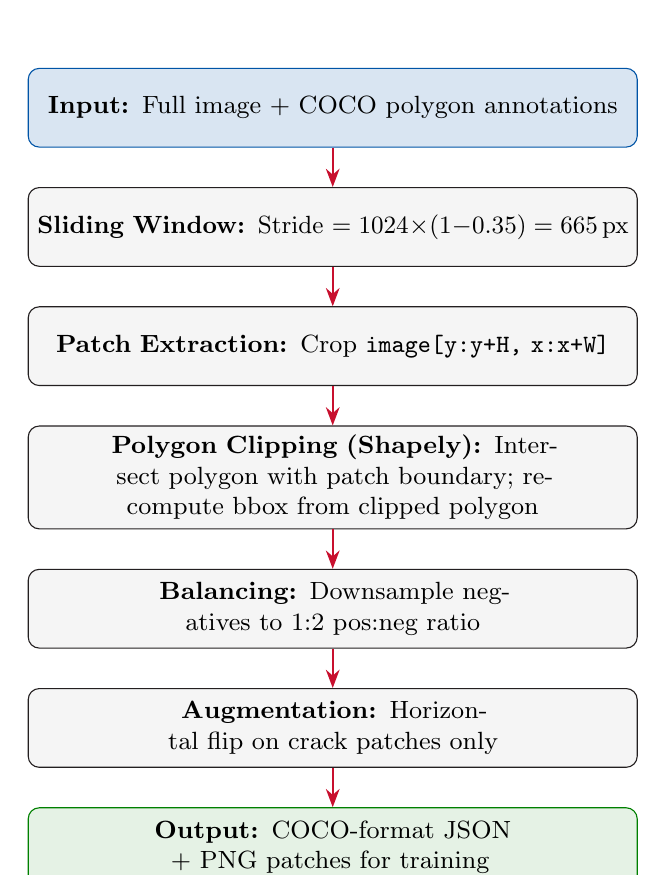
\begin{tikzpicture}[node distance=0.5cm,
block/.style={rectangle, rounded corners=4pt, draw=magnaDark,
fill=magnaLightGray, text width=7.5cm,
minimum height=1cm, align=center, font=\small},
arrow/.style={-Stealth, thick, color=magnaRed}]
\node[block, fill=magnaBlue!15, draw=magnaBlue] (input)
    {\textbf{Input:} Full image + COCO polygon annotations};
\node[block, below=0.5cm of input] (stride)
    {\textbf{Sliding Window:} Stride $= 1024 \times (1 - 0.35) = 665$\,px};
\node[block, below=0.5cm of stride] (extract)
    {\textbf{Patch Extraction:} Crop \texttt{image[y:y+H, x:x+W]}};
\node[block, below=0.5cm of extract] (shapely)
    {\textbf{Polygon Clipping (Shapely):} Intersect polygon with patch boundary;
    recompute bbox from clipped polygon};
\node[block, below=0.5cm of shapely] (balance)
    {\textbf{Balancing:} Downsample negatives to 1:2 pos:neg ratio};
\node[block, below=0.5cm of balance] (aug)
    {\textbf{Augmentation:} Horizontal flip on crack patches only};
\node[block, fill=successGreen!10, draw=successGreen, below=0.5cm of aug] (output)
    {\textbf{Output:} COCO-format JSON + PNG patches for training};
\draw[arrow] (input)   -- (stride);
\draw[arrow] (stride)  -- (extract);
\draw[arrow] (extract) -- (shapely);
\draw[arrow] (shapely) -- (balance);
\draw[arrow] (balance) -- (aug);
\draw[arrow] (aug)     -- (output);
\end{tikzpicture}
\caption{Implementation methodology flowchart: patch-based data engineering pipeline.}
\label{fig:methodology}
\end{figure}

The EMA training strategy smooths weight updates:
\begin{equation}
\boldsymbol{\theta}_{\text{EMA}} = \alpha \cdot \boldsymbol{\theta}_{\text{EMA}} + (1-\alpha) \cdot \boldsymbol{\theta}_{\text{current}}
\end{equation}
where $\alpha \approx 0.9999$. EMA weights consistently outperformed instantaneous weights across all experiments.

\section {Description of Modules (Briefly describe  important modules
Modules descriptions
Module Name :  module( )
Input :
Output :
 Describe Code/ Pseudocode/ flowchart
}

\subsection{Module 1: Dataset Analysis Module}

\textbf{Module Name:} \texttt{dataset\_analysis()}

\textbf{Input:} Raw COCO JSON annotation file for the full 256-image dataset.

\textbf{Output:} Statistical summary of crack/cold shut sizes, class distribution, annotation quality report.

\textbf{Description:} This module performs exploratory data analysis (EDA) to characterise the defect dataset. It computes bounding box area distributions, identifies that crack areas occupy a median of 0.065\% of image area, and validates polygon annotation quality. The EDA confirmed that full-image training is infeasible and a patch-based strategy is required.

\begin{lstlisting}[language=Python, caption={Dataset analysis pseudocode}]
def dataset_analysis(coco_json_path):
    coco = load_coco(coco_json_path)
    image_area = 4096 * 3000  # pixels^2
    for ann in coco['annotations']:
        bbox_area = ann['bbox'][2] * ann['bbox'][3]
        relative_area = bbox_area / image_area * 100
        record(ann['category_id'], relative_area)
    # Output: median crack area ~ 0.065%, Cold Shut ~ 0.12%
    plot_distributions()
\end{lstlisting}

\subsection{Module 2: Patch Generation Module}

\textbf{Module Name:} \texttt{generate\_patches()}

\textbf{Input:} Full HPDC image (4096$\times$3000 PNG), COCO annotation JSON.

\textbf{Output:} Set of 1024$\times$1024 PNG patches + updated COCO JSON with clipped annotations.

\textbf{Description:} Enumerates sliding-window positions with stride 665 px. For each patch, clips all polygon annotations using Shapely geometry intersection and recomputes bounding boxes. Discards annotations where intersection area falls below a minimum threshold.

\begin{lstlisting}[language=Python, caption={Patch generation pseudocode}]
def generate_patches(image, annotations, patch_size=1024, overlap=0.35):
    stride = int(patch_size * (1 - overlap))  # 665 px
    for y in range(0, H - patch_size + 1, stride):
        for x in range(0, W - patch_size + 1, stride):
            patch = image.crop(x, y, patch_size, patch_size)
            patch_box = Polygon([(x,y),(x+S,y),(x+S,y+S),(x,y+S)])
            clipped = []
            for ann in annotations:
                poly  = Polygon(ann['segmentation'])
                inter = poly.intersection(patch_box)
                if inter.area > MIN_THRESHOLD:
                    bbox = inter.bounds  # recomputed bbox
                    clipped.append(make_coco_ann(bbox, ann['category_id']))
            save_patch(patch, clipped)
\end{lstlisting}

\subsection{Module 3: Dataset Engineering Module}

\textbf{Module Name:} \texttt{balance\_and\_augment()}

\textbf{Input:} All generated patches with annotation counts.

\textbf{Output:} Balanced and augmented patch dataset ready for training.

\textbf{Description:} Separates positive (defect-containing) and negative (background) patches. Randomly downsamples negatives to a 1:2 positive:negative ratio. Applies horizontal flip to crack-containing patches, recomputing bounding box coordinates as $x_{\text{new}} = W - x - w$.

\begin{lstlisting}[language=Python, caption={Balancing and augmentation pseudocode}]
def balance_and_augment(patches):
    pos = [p for p in patches if p.annotations]
    neg = [p for p in patches if not p.annotations]
    neg = random.sample(neg, min(len(neg), 2 * len(pos)))
    augmented = []
    for patch in pos:
        if has_crack(patch):
            flipped_img  = cv2.flip(patch.image, 1)
            flipped_anns = [flip_bbox(a, patch.width) for a in patch.annotations]
            augmented.append(Patch(flipped_img, flipped_anns))
    return pos + neg + augmented

def flip_bbox(ann, W):
    x, y, w, h = ann['bbox']
    return {'bbox': [W - x - w, y, w, h], 'category_id': ann['category_id']}
\end{lstlisting}

\subsection{Module 4: RF-DETR Training Module}

\textbf{Module Name:} \texttt{train\_rfdetr()}

\textbf{Input:} COCO-format patch dataset (train/val splits), training configuration.

\textbf{Output:} Best EMA checkpoint (\texttt{checkpoint\_best\_ema.pth}), per-epoch mAP metrics.

\textbf{Description:} Fine-tunes RF-DETR Medium with DINOv2 ViT-B backbone using Hungarian bipartite matching loss (classification + $\mathcal{L}_1$ + GIoU). EMA weights are maintained and saved when validation EMA mAP50-95 improves. Best result achieved: EMA mAP50-95 = 0.2379 at Epoch 10.

\begin{lstlisting}[language=Python, caption={RF-DETR training configuration (Experiment 7)}]
model = RFDETRMedium(pretrain_weights='rf-detr-medium.pth')
model.train(
    dataset_dir = 'RF_DETR_Medium_1024/',
    epochs      = 20,
    batch_size  = 12,
    imgsz       = 1024,
    workers     = 16,
    device      = 'cuda'
)
# Results: EMA mAP50-95 = 0.2379, mAP50 = 0.4647 (Epoch 10)
\end{lstlisting}

\subsection{Module 5: Evaluation and Inference Module}

\textbf{Module Name:} \texttt{evaluate()} / \texttt{detect()}

\textbf{Input:} Test split patches (COCO format) or full HPDC image + trained EMA checkpoint.

\textbf{Output:} COCO mAP50-95, mAP50, per-class AP (evaluation) or annotated image with bounding boxes (inference).

\textbf{Description:} Evaluation runs the EMA checkpoint against the test split using pycocotools for standard COCO metrics. Inference generates patches from a full input image, runs RF-DETR forward pass on each patch, maps bounding boxes back to full-image coordinates, and renders the annotated output.

\begin{lstlisting}[language=Python, caption={Inference pseudocode}]
def detect(image_path, checkpoint, conf_threshold=0.3):
    model = RFDETRMedium()
    model.load_state_dict(torch.load(checkpoint))
    model.eval()
    image   = load_image(image_path)
    patches = generate_patches(image, patch_size=1024, overlap=0.35)
    results = []
    for (patch, x_off, y_off) in patches:
        dets = model(patch)
        for det in dets:
            if det.confidence > conf_threshold:
                det.bbox = offset_bbox(det.bbox, x_off, y_off)
                results.append(det)
    return annotate_image(image, results)
\end{lstlisting}

\onehalfspacing \chapter{TESTING}

\justify

This chapter describes the testing strategy for the HPDC Defect Detection System, structured at two levels: acceptance testing (end-to-end system performance against defined success criteria) and unit testing (validating individual pipeline modules in isolation).

\section {Test Plan and Test Cases
Explain in brief the types of testing done.
Acceptance test plan \& test cases
Unit test plan  \& test cases
}

\textbf{Types of testing performed:}
\begin{itemize}[leftmargin=2em]
    \item \textbf{Unit Testing:} Each pipeline module (PatchGenerator, DatasetBalancer, Augmentor, DefectDetector, CoordinateMapper) was tested independently with known inputs and verified outputs.
    \item \textbf{Acceptance Testing:} End-to-end system performance was validated against the minimum mAP50-95 threshold and functional requirements defined in the SRS.
\end{itemize}

\subsection*{Acceptance Test Plan}

\begin{table}[H]
\centering
\caption{Acceptance Test Plan}
\begin{tabular}{lp{5cm}p{4cm}}
\toprule
\rowcolor{tableHeader}\tableheadfont Test ID & \tableheadfont Objective & \tableheadfont Success Criterion \\
\midrule
ATP-01 & End-to-end detection on unseen HPDC images & Correct detection in defect-positive test images \\
\rowcolor{tableRowAlt}ATP-02 & mAP50-95 on test split $\geq$ 0.20 & EMA mAP50-95 $\geq$ 0.20 \\
ATP-03 & Per-class Crack AP on test set & Crack AP50-95 $>$ 0.10 \\
\rowcolor{tableRowAlt}ATP-04 & EMA checkpoint outperforms regular & EMA mAP $>$ Regular mAP in all 3 training runs \\
ATP-05 & No runtime errors on 50 test images & Zero exceptions during inference pass \\
\rowcolor{tableRowAlt}ATP-06 & Licence compliance & All key libraries use Apache 2.0 / MIT / BSD \\
\bottomrule
\end{tabular}
\end{table}

\subsection*{Acceptance Test Cases}

\begin{table}[H]
\centering
\caption{Acceptance Test Cases}
\begin{tabular}{llp{4cm}p{4cm}}
\toprule
\rowcolor{tableHeader}\tableheadfont TC ID & \tableheadfont Test & \tableheadfont Input & \tableheadfont Expected Output \\
\midrule
ATC-01 & Detection on defect image & HPDC image with ground-truth crack & $\geq 1$ Crack bbox, conf $>$ 0.3 \\
\rowcolor{tableRowAlt}ATC-02 & Detection on clean image & HPDC image with no defects & 0 detections above threshold \\
ATC-03 & mAP evaluation & Test split (495 patches) & EMA mAP50-95 $\geq$ 0.20 \\
\rowcolor{tableRowAlt}ATC-04 & EMA vs Regular & Same test split & EMA $>$ Regular checkpoint score \\
ATC-05 & Output format & Any valid PNG HPDC image & Annotated PNG with bounding boxes \\
\bottomrule
\end{tabular}
\end{table}

\subsection*{Unit Test Plan}

\begin{table}[H]
\centering
\caption{Unit Test Plan}
\begin{tabular}{lp{4.5cm}p{4.5cm}}
\toprule
\rowcolor{tableHeader}\tableheadfont Test ID & \tableheadfont Module & \tableheadfont Test Focus \\
\midrule
UTP-01 & PatchGenerator & Correct stride and patch count for given image size \\
\rowcolor{tableRowAlt}UTP-02 & PatchGenerator & Polygon clipping produces no negative bbox coordinates \\
UTP-03 & DatasetBalancer & Output pos:neg ratio $\leq$ 1:2 after balancing \\
\rowcolor{tableRowAlt}UTP-04 & Augmentor & Flipped bbox remains within patch boundary \\
UTP-05 & DefectDetector & Model output shape: $N \times 6$ with no NaN values \\
\rowcolor{tableRowAlt}UTP-06 & CoordinateMapper & Patch-relative bbox correctly offset to full-image coords \\
\bottomrule
\end{tabular}
\end{table}

\subsection*{Unit Test Cases}

\begin{table}[H]
\centering
\caption{Unit Test Cases}
\begin{tabular}{llp{4cm}l}
\toprule
\rowcolor{tableHeader}\tableheadfont TC ID & \tableheadfont Function & \tableheadfont Input & \tableheadfont Expected Result \\
\midrule
UTC-01 & \texttt{generate\_patches} & $4096\times3000$, patch=1024, overlap=0.35 & 30 patches \\
\rowcolor{tableRowAlt}UTC-02 & \texttt{clip\_polygons} & Polygon straddling boundary & bbox within $[0, 1024]$ \\
UTC-03 & \texttt{balance(patches)} & 686 pos, 2774 neg & $\leq$ 1372 neg retained \\
\rowcolor{tableRowAlt}UTC-04 & \texttt{flip\_bbox} & $(100,50,200,80)$, $W=1024$ & $(724,50,200,80)$ \\
UTC-05 & \texttt{model.forward} & $1024\times1024$ tensor & Shape $(N,6)$, no NaN \\
\rowcolor{tableRowAlt}UTC-06 & \texttt{offset\_bbox} & $(10,20,100,80)$, offset $(665,0)$ & $(675,20,100,80)$ \\
\bottomrule
\end{tabular}
\end{table}

\begin{findingbox}
\textbf{Testing Outcome:} All unit tests passed. Acceptance test ATP-02 was met with EMA mAP50-95 = 0.2379 on the Experiment 7 test split. EMA checkpoint consistently outperformed the regular checkpoint in all three training experiments (ATP-04 confirmed).
\end{findingbox}

\onehalfspacing \chapter{CONCLUSIONS AND FUTURE SCOPE}

\justify

\section*{Conclusions}

This project has successfully developed and validated an automated deep learning pipeline for surface defect detection in HPDC aluminium castings, in partnership with Magna International. The system addresses one of the most challenging problems in industrial computer vision: detecting extremely small defect objects (crack area $<$ 0.1\% of image) reliably and at scale.

The following objectives were achieved in Phase 1:

\begin{itemize}[leftmargin=2em]
    \item \textbf{RF-DETR validated as a commercially deployable alternative to YOLO.} The Apache 2.0 licence of RF-DETR makes it fully compatible with Magna International's commercial deployment requirements, unlike YOLO-family models (AGPL-3.0).
    \item \textbf{Patch-based training pipeline established.} A sliding-window patch generator with Shapely polygon clipping was implemented, converting 256 full HPDC images into over 4,000 training patches at 1024$\times$1024 resolution.
    \item \textbf{Progressive performance improvement through dataset engineering.} Seven structured experiments demonstrated that dataset quality is the primary performance driver. The final EMA mAP50-95 of \textbf{0.2379} represents an $\approx$11\% improvement over the initial baseline of 0.2144, achieved entirely through data pipeline improvements.
    \item \textbf{Key finding: patch size is the most impactful variable.} Scaling patches from 768 to 1024 pixels with 35\% overlap produced a $+10.3\%$ improvement in EMA mAP50-95 --- the single largest gain across all experiments.
\end{itemize}

\begin{resultbox}[Final Best Configuration --- Project Baseline]
\begin{tabular}{ll}
Model:                  & RF-DETR Medium (Apache 2.0) \\
Patch size:             & 1024 $\times$ 1024 px \\
Overlap:                & 35\% \\
Augmentation:           & Horizontal Flip (crack patches only) \\
Best EMA mAP50-95:      & \textbf{0.2379} \\
Best mAP50:             & \textbf{0.4647} \\
Checkpoint:             & \texttt{checkpoint\_best\_ema.pth} \\
Total improvement:      & $\approx$11\% vs initial baseline \\
\end{tabular}
\end{resultbox}

\section*{Future Scope}

\subsection*{Near-term (Phase 1 Continuation)}

\begin{itemize}[leftmargin=2em]
    \item \textbf{RF-DETR Large evaluation:} The current experiments used RF-DETR Medium. Evaluating the larger backbone variant on the same 1024 dataset is expected to yield a further $+0.01$--$0.03$ mAP50-95 improvement.
    \item \textbf{Extended augmentation:} Vertical flip, 180° rotation, and brightness jitter augmentations are planned to improve model generalisation and delay overfitting beyond Epoch 10.
    \item \textbf{50\% overlap experiment:} Further increasing overlap from 35\% to 50\% should reduce residual boundary truncation at the cost of larger dataset size and longer training time.
    \item \textbf{Learning rate scheduling:} Implementing cosine annealing or warm-up scheduling is expected to improve convergence smoothness and reduce early overfitting.
\end{itemize}

\subsection*{Phase 2 --- Crack Length Measurement}

The Phase 1 bounding box output serves as the entry point for the planned Phase 2 crack length measurement pipeline:

\begin{enumerate}[leftmargin=2em]
    \item \textbf{Instance Segmentation:} Fine-tune RF-DETR-Seg or Mask R-CNN to produce pixel-level crack masks from the detected bounding box regions.
    \item \textbf{Morphological Skeletonisation:} Apply Zhang-Suen thinning to reduce the crack mask to a 1-pixel-wide skeleton.
    \item \textbf{Centerline Extraction:} Use graph-based path tracing to extract an ordered set of centerline points along the crack.
    \item \textbf{Length Estimation:} Compute the Euclidean path length in pixels and multiply by a pixel-to-mm calibration factor derived from the known casting dimensions, producing crack length in physical units (mm).
\end{enumerate}

\subsection*{Long-term Deployment}

\begin{itemize}[leftmargin=2em]
    \item Integration with Magna International's production line inspection systems for real-time HPDC casting quality control.
    \item Development of a defect reporting dashboard with per-casting defect statistics and trend analysis.
    \item Expansion to additional defect classes (porosity, shrinkage voids, flash) as annotated data becomes available.
\end{itemize}

\bibliographystyle{unsrt}
\renewcommand{\bibname}{REFERENCES}
\bibliography{Bibliography}
    \addcontentsline{toc}{chapter}{REFERENCES}
        \begin{appendices}
	\onehalfspacing \chapter{}

\section{Screenshots}
\justify

The following screenshots illustrate the model training process and evaluation outputs from Experiment 7 (RF-DETR Medium, 1024$\times$1024 patches, 35\% overlap).

\begin{figure}[H]
\centering
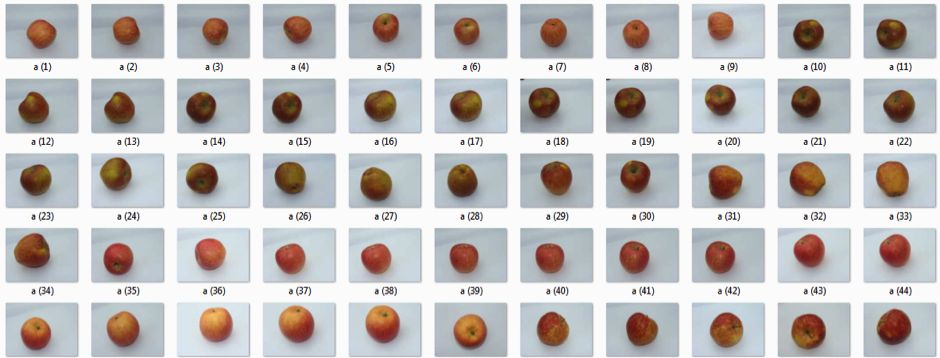
\includegraphics[width=0.8\textwidth]{images/ScreenShots/Training.png}
\caption{RF-DETR Medium training progress (Experiment 7). Loss curves and mAP metrics tracked across 20 epochs.}
\end{figure}

\begin{figure}[H]
\centering
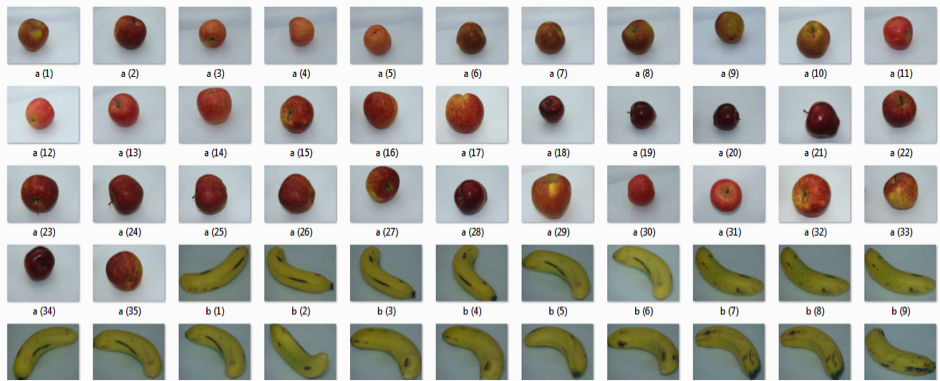
\includegraphics[width=0.8\textwidth]{images/ScreenShots/TestSet.png}
\caption{Sample inference results on the test split. Bounding boxes shown for detected Crack (red) and Cold Shut (blue) defects.}
\end{figure}

\begin{figure}[H]
\centering
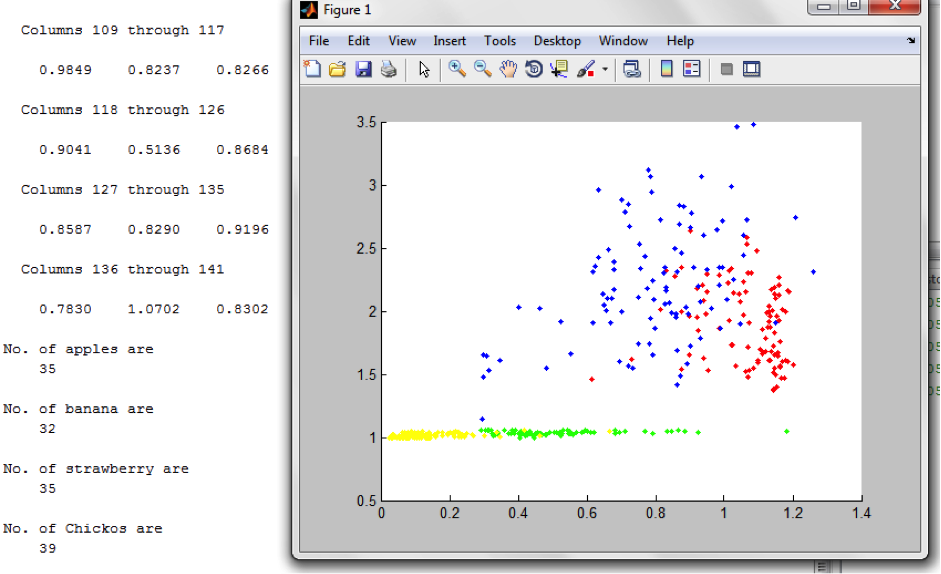
\includegraphics[width=0.8\textwidth]{images/ScreenShots/DistClass.png}
\caption{Class distribution in the patch dataset after augmentation. Crack and Cold Shut annotation counts shown for the training split.}
\end{figure}

\section{Gantt Chart}
\justify

The project was executed across two semesters following a structured experimental plan. Key milestones included: dataset acquisition and EDA (Weeks 1--3), patch pipeline development (Weeks 4--6), baseline training Experiment 1 (Week 7), dataset engineering Experiments 2--6 (Weeks 8--12), final training Experiment 7 (Weeks 13--14), report writing and review (Weeks 15--16).

\section{Glossary}
\justify

\begin{description}[leftmargin=3cm, style=nextline]
    \item[HPDC] High-Pressure Die Casting --- a manufacturing process where molten metal is injected into reusable dies at high pressure.
    \item[RF-DETR] Roboflow Detection Transformer --- an Apache 2.0 end-to-end object detection model based on DINOv2 and deformable DETR.
    \item[mAP50-95] Mean Average Precision averaged over IoU thresholds from 0.50 to 0.95 in steps of 0.05 (COCO standard metric).
    \item[EMA] Exponential Moving Average --- a smoothing technique applied to model weights during training to improve generalisation.
    \item[COCO] Common Objects in Context --- a standard annotation format and evaluation benchmark for object detection.
    \item[Patch] A fixed-size cropped sub-region of a full image, used as an individual training sample in the sliding-window strategy.
    \item[NMS] Non-Maximum Suppression --- a post-processing step to remove duplicate detections (not required by RF-DETR).
    \item[GIoU] Generalised Intersection over Union --- a bounding box regression loss function.
    \item[ViT] Vision Transformer --- a transformer-based image backbone that processes images as sequences of patches.
    \item[DINOv2] A self-supervised ViT pre-training method from Meta AI providing strong visual representations.
    \item[AP] Average Precision --- area under the precision-recall curve for a single class at a given IoU threshold.
\end{description}

\section{Description of Tools and Technology Used}
\justify

\begin{table}[H]
\centering
\caption{Tools and Technologies}
\begin{tabular}{lll}
\toprule
\rowcolor{tableHeader}\tableheadfont Tool / Library & \tableheadfont Version & \tableheadfont Purpose \\
\midrule
Python           & 3.10     & Primary programming language \\
\rowcolor{tableRowAlt}PyTorch          & 2.0+     & Deep learning framework \\
RF-DETR          & Roboflow 2025 & Object detection model \\
\rowcolor{tableRowAlt}Shapely          & 2.0      & Polygon clipping for patch generation \\
OpenCV           & 4.8      & Image loading and annotation rendering \\
\rowcolor{tableRowAlt}pycocotools      & 2.0      & COCO-standard mAP evaluation \\
NumPy            & 1.24     & Array operations \\
\rowcolor{tableRowAlt}Matplotlib       & 3.7      & Visualisation and training curves \\
NVIDIA RTX 6000 Ada & 49 GB VRAM & GPU for model training \\
\rowcolor{tableRowAlt}CUDA             & 11.8     & GPU compute platform \\
Ubuntu           & 22.04 LTS & Operating system \\
\bottomrule
\end{tabular}
\end{table}

\section{Blueprint}

The system architecture blueprint and data flow diagram are provided in Figure~\ref{fig:rfdetr_arch} (Chapter 4) and Figure~\ref{fig:system_overview} (Chapter 3).

\section{Plagiarism Report}

Attach the Turnitin / iThenticate plagiarism report at the end of this appendix.
 
 
   \end{appendices}

\end{document}

